\subsection{Separate Bewegungsabläufe}

Das erste Ziel ist es, dem Läufer das Stehenbleiben beizubringen. Hierfür soll der Läufer sich möglichst wenig von der aktuellen Position wegbewegen, wobei die Hauptaufgabe darin besteht, das Gleichgewicht zu halten.

Um das Stehenbleiben zu erreichen, wird die Zielgeschwindigkeit auf 0 gesetzt, während das Ziel an der Startposition bleibt. Eine Herausforderung hierbei ist die ursprüngliche Demo-Belohnungsfunktion, die durch die Zielgeschwindigkeit dividiert. Da dies bei einer Zielgeschwindigkeit von 0 zu mathematischen Fehlern führt, war eine Anpassung der Belohnungsfunktion notwendig. Statt der ursprünglichen Funktion wurde eine alternative Belohnungsfunktion implementiert, um das Problem zu beheben. Es wird erwartet, dass die Neue Belohnungsfunktion die Lernfähigkeit des Modells verbessert, auf der Stelle zu stehen, ohne zu fallen. Es muss jedoch auch untersucht werden wie die Neue Belohnungsfunktion die Lernfähigkeit des ursprünglichen Verhaltens beeinflusst.

\begin{figure}[H]
  \centering  
  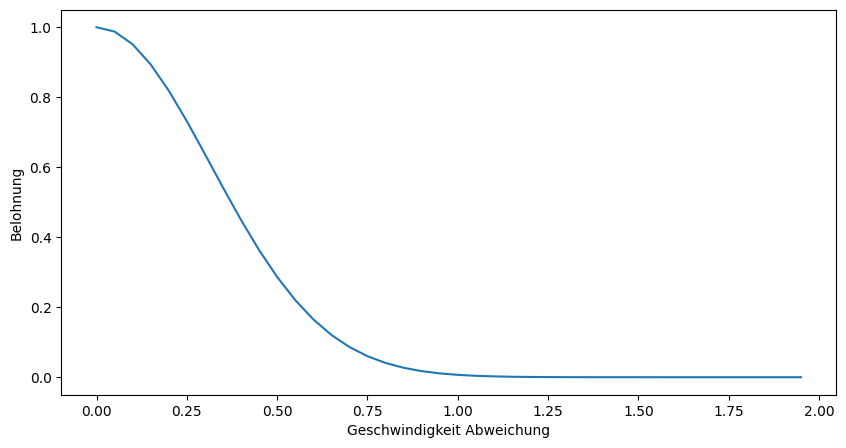
\includegraphics[width=0.85\textwidth]{img/plot_vel_reward_neu}
  \caption{Neue Sigmoid Geschwindigkeitbelohnungsfunktion}
  \label{fig:plot_vel_reward_neu}
\end{figure}

Als Neue Belohnungsfunktion wird eine Sigmoid-Funktion genutzt, die eine glatte Abstufung der Belohnungen ermöglicht. Die Belohnung erreicht den Wert 1, wenn die aktuelle Geschwindigkeit perfekt mit der Zielgeschwindigkeit übereinstimmt. Mit zunehmender Abweichung von der Zielgeschwindigkeit sinkt die Belohnung stetig, und sobald die Abweichung den Wert 1 überschreitet, fällt die Belohnung auf 0. Die Belohnungsfunktion und ihre Parameter wurden so gewählt, dass die Neue Belohnungsfunktion der Demo Belohnungsfunktion ähnelt. Die Neue Belohnungsfunktion abgebildet in Abbildung \ref{fig:plot_vel_reward_neu} wird daher ab hier Neue Belohnungsfunktion genannt.

Der Walker konnte mit der Neuen Belohnungsfunktion erfolgreich lernen, auf der Stelle zu stehen. Dies wird in den Abbildungen \ref{fig:126_episode_length} und \ref{fig:126_move_target_dir} verdeutlicht. Die Abbildung \ref{fig:126_move_target_dir} zeigt, wie die zurückgelegte Distanz um 0 herum schwankt, was darauf hinweist, dass der Läufer in der Lage ist, seine Position zu halten. Gleichzeitig erreicht die Episodenlänge in Abbildung \ref{fig:126_episode_length} die maximale Länge von 1000, was bedeutet, dass der Läufer über die gesamte Episode hinweg stabil blieb.
\begin{figure}[H]
  \centering  
  \begin{subfigure}{.49\textwidth}
      \centering  
      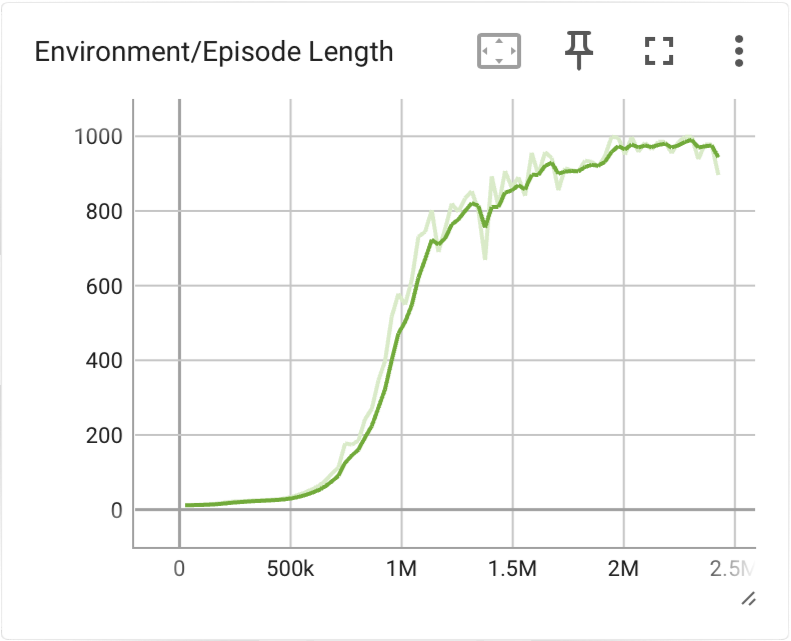
\includegraphics[width=\textwidth]{img/126_episode_length}
      \caption{Episodenlänge}
      \label{fig:126_episode_length}
    \end{subfigure}
    \begin{subfigure}{.49\textwidth}
      \centering  
      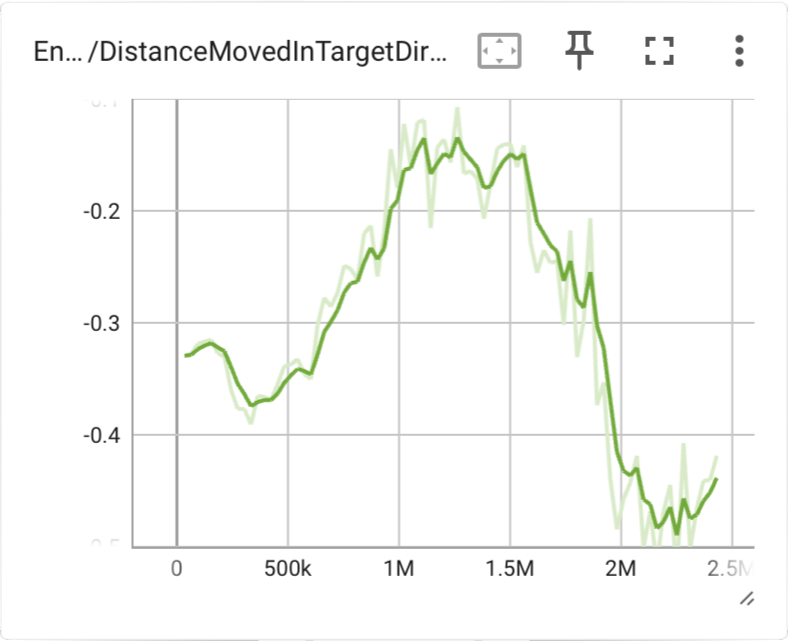
\includegraphics[width=\textwidth]{img/126_move_target_dir}
      \caption{Zurückgelegte Stecke in Zielrichtung}
      \label{fig:126_move_target_dir}
    \end{subfigure}
  \caption{Training stehen mit neuer Belohnungsfunktion}
  \label{fig:training_stehen_neu}
\end{figure}

Mit zufälliger Zielgeschwindigkeit zu einem Ziel zu laufen, wie es im ursprünglichen Verhalten vorgesehen war, konnte jedoch mit der Neuen Belohnungsfunktion nicht zufriedenstellend erlernt werden. In Abbildung \ref{fig:training_vergleich_demo_neu} ist die Leistung der Neuen Belohnungsfunktion durch die orangene Linie und die Leistung der Demo-Belohnungsfunktion durch die rosa Linie dargestellt. Die Abbildung \ref{fig:match_velocity_demo_vergleich} zeigt, dass die ursprüngliche Belohnungsfunktion die Fehlertoleranz in Abhängigkeit von der Zielgeschwindigkeit dynamisch anpasst, was dem Modell ermöglicht, besser zwischen unterschiedlichen Geschwindigkeiten zu generalisieren. Die Ergebnisse zeigen, dass während die Neue Belohnungsfunktion gut für das Erlernen der Stabilisierung des Läufers auf der Stelle ist, die ursprüngliche Belohnungsfunktion sich besser für das Erlernen einer Gangbewegung in Zielrichtung eignet.

\begin{figure}[H]
  \centering  
  \begin{subfigure}{.49\textwidth}
      \centering  
      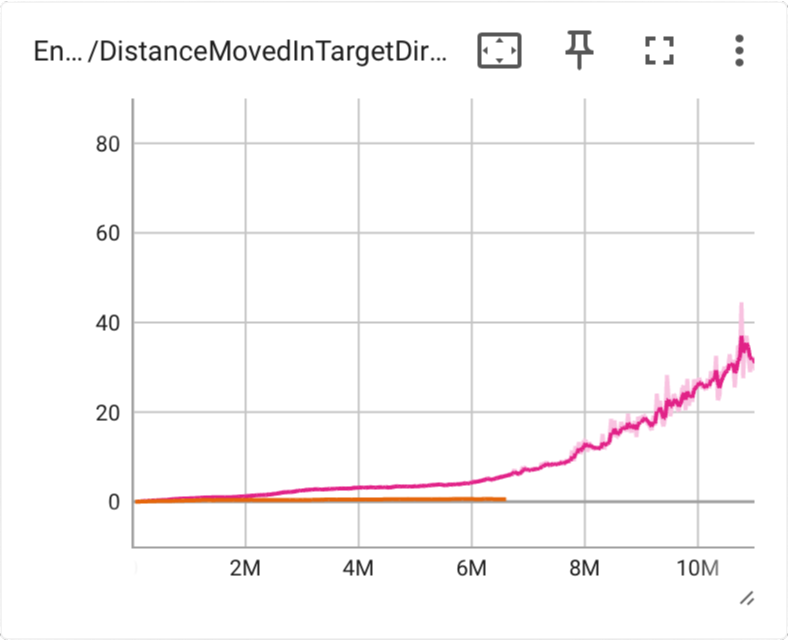
\includegraphics[width=\textwidth]{img/116_127_move_target_dir}
      \caption{Zurückgelegte Stecke in Zielrichtung}
      \label{fig:116_127_move_target_dir}
    \end{subfigure}
    \begin{subfigure}{.49\textwidth}
      \centering  
      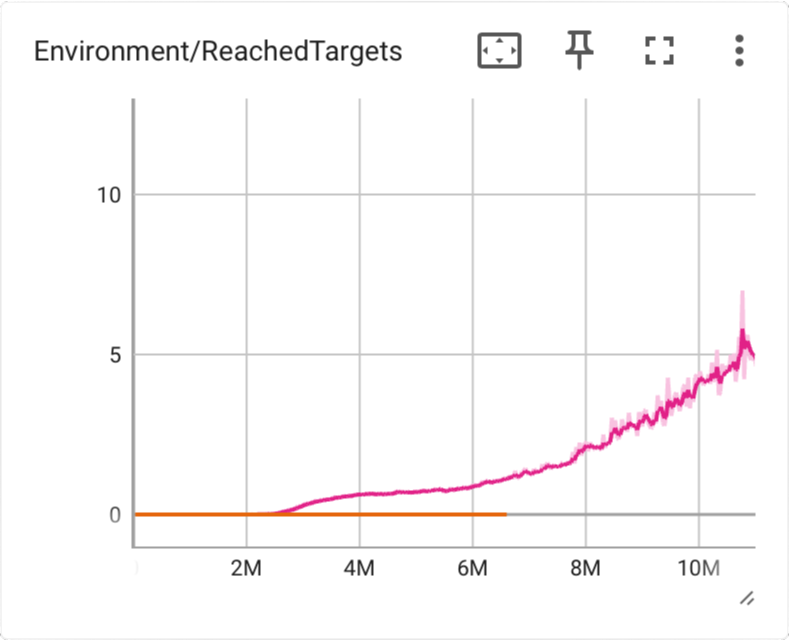
\includegraphics[width=\textwidth]{img/116_127_reach_target}
      \caption{Anzahl erreichte Ziele}
      \label{fig:116_127_reach_target}
    \end{subfigure}
  \caption{Vergleich von Lauftraining mit Demo Belohnungsfunktion gegen Neue Belohnungsfunktion}
  \label{fig:training_vergleich_demo_neu}
\end{figure}

\begin{figure}[H]
  \centering  
  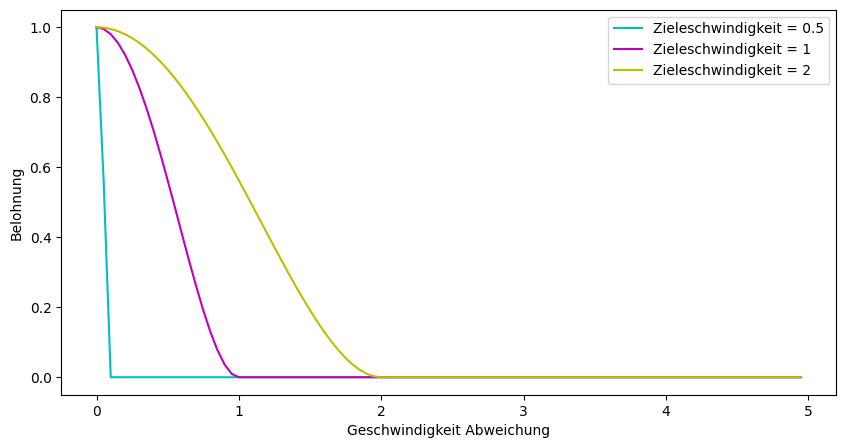
\includegraphics[width=0.9\textwidth]{img/match_velocity_demo_vergleich}
  \caption{Vergleich der Demo Belohnungsfunktion unter verschiedenen Zielgeschwindigkeiten}
  \label{fig:match_velocity_demo_vergleich}
\end{figure}

Mit dieser Erkenntnis wird eine neue Anpassung untersucht. In der folgenden Anpassung bleibt die Belohnungsfunktion weitestgehend unverändert; lediglich das obere Limit, ab welchem die Funktion eine Belohnung von 0 annimmt, wird auf ein Minimum von 0,1 beschränkt. Diese Anpassung stellt sicher, dass im Bereich der normalen Fortbewegung keine unerwünschten Veränderungen auftreten. Das Problem mit der ursprünglichen Demo-Belohnungsfunktion bestand darin, dass bei Annäherung an eine Zielgeschwindigkeit von 0 das Spektrum an akzeptablen Geschwindigkeiten, bevor die Belohnung auf 0 sinkt, extrem eng wurde (siehe Abbildung \ref{fig:match_velocity_vergleich_clip}). Dies machte es nahezu unmöglich, sinnvolle Lernfortschritte in diesem Bereich zu erzielen. Durch die Einführung eines Limits von 0,1 wird der Bereich der Geschwindigkeitsabweichungen, für die die Belohnungsfunktion einen Wert größer 0 annimmt, ausreichend vergrößert. Dies ermöglicht dem Läufer, durch Ausprobieren Belohnungen über 0 zu erreichen, was wiederum eine Richtung für die Optimierung des Verhaltens bietet. Somit kann der Läufer die Belohnung optimieren.

\begin{figure}[H]
  \centering  
  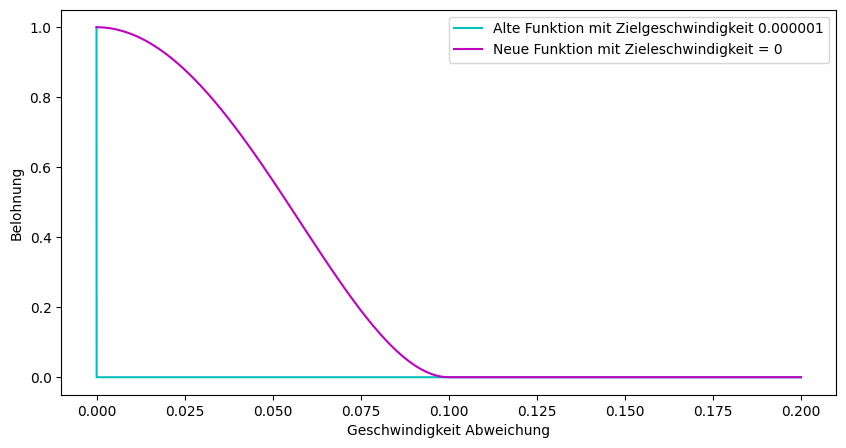
\includegraphics[width=0.9\textwidth]{img/match_velocity_vergleich_clip}
  \caption{Vergleich Demo gegen Belohnungsfunktion mit 0.1 Limit}
  \label{fig:match_velocity_vergleich_clip}
\end{figure}

Mit der angepassten Demo-Belohnungsfunktion konnte nach etwas mehr Trainingsschritten ebenfalls die maximale Episodenlänge von 1000 erreicht werden (siehe Abbildung \ref{fig:126_128_episode_length}. Dies zeigt, dass der Läufer in der Lage war, über eine längere Trainingsdauer hinweg die erforderliche Stabilität zu erlernen. Die in Abbildung \ref{fig:126_128_move_target_dir} dargestellte zurückgelegte Distanz nähert sich gegen Ende fast 0, was darauf hindeutet, dass der Läufer seine Position sehr gut halten kann. Dieses Ergebnis zeigt, dass auch mit der angepassten Demo-Belohnungsfunktion ein vergleichbares Niveau an Stabilität erreicht werden kann, ohne den Lernvorgang für das ursprüngliche Verhalten zu beeinflussen.

\begin{figure}[H]
  \centering  
  \begin{subfigure}{.49\textwidth}
      \centering  
      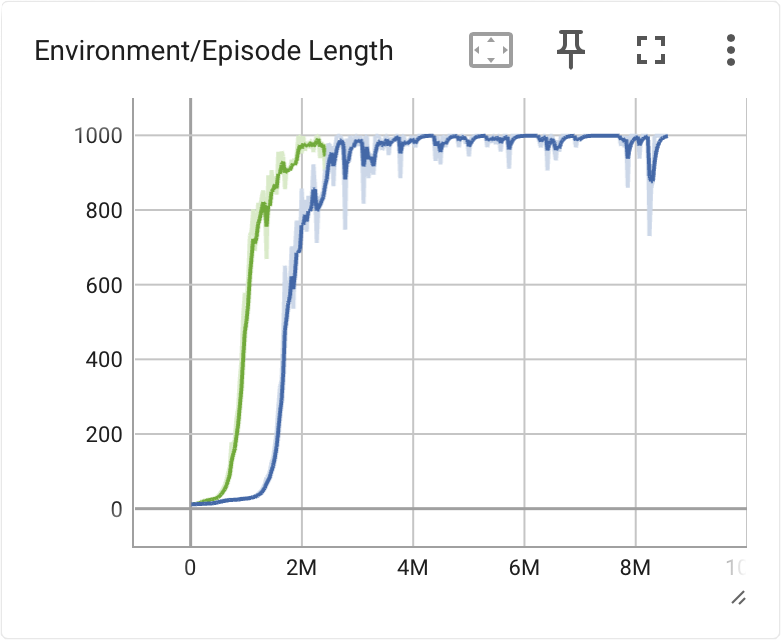
\includegraphics[width=\textwidth]{img/126_128_episode_length}
      \caption{Episodenlänge}
      \label{fig:126_128_episode_length}
    \end{subfigure}
    \begin{subfigure}{.49\textwidth}
      \centering  
      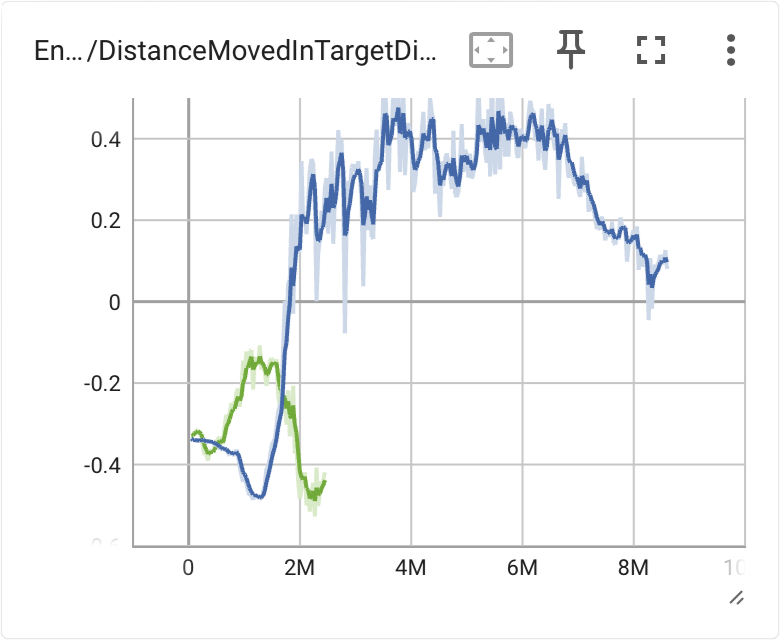
\includegraphics[width=\textwidth]{img/126_128_move_target_dir}
      \caption{Zurückgelegte Stecke in Zielrichtung}
      \label{fig:126_128_move_target_dir}
    \end{subfigure}
  \caption{Vergleich Training stehen mit Neuer Belohnungfunktion (orange) und angepasster Demo Belohnungsfunktion (blau)}
  \label{fig:vergleich_126_128}
\end{figure}

Nach dem erfolgreichen Erlernen des Stehens auf einer festen Position sind die nächsten Bewegungsziele die Fortbewegung zum Ziel mit unterschiedlichen Blickrichtungen. Die Extremfälle umfassen dabei das Rückwärts- und Seitwärtslaufen. In diesem Abschnitt wird untersucht, ob der Läufer in der Lage ist, Bewegungen in verschiedene Richtungen relativ zu seiner Blickrichtung zu erlernen. Um dies zu ermöglichen, wurde die Belohnungsfunktion angepasst, sodass sie die Blickrichtung relativ zur Zielrichtung berücksichtigt. Bei der Vorwärtsbewegung entspricht die Blickrichtung der Zielrichtung. Bei der Seitwärtsbewegung steht die Blickrichtung im rechten Winkel zur Zielrichtung, und bei der Rückwärtsbewegung ist die Blickrichtung entgegengesetzt zur Zielrichtung. Die Implementierung zur Bestimmung der Blickrichtung ist in \ref{lst:blickrichtung} dargestellt.

\begin{lstlisting}[caption={Blickrichtung festlegen mit Richtungs Enum},captionpos=b,label={lst:blickrichtung}]
public enum Direction
{
    Forward,
    Right,
    Left,
    Backward,
}
    
public override void FixedUpdate()
{
    ...
    var headForward = head.forward;
    headForward.y = 0;
    Vector3 lookDirection = cubeForward;
    switch (direction)
    {
        case Direction.Right:
            lookDirection = -walkOrientationCube.transform.right;
            break;
        case Direction.Left:
            lookDirection = walkOrientationCube.transform.right;
            break;
        case Direction.Backward:
            lookDirection = -walkOrientationCube.transform.forward;
            break;
    }
    var lookAtTargetReward = (Vector3.Dot(lookDirection, headForward) + 1) * 0.5F;
    ...
}
\end{lstlisting}

Das Gehen in Zielrichtung wurde durch die Änderungen nicht negativ beeinflusst. Separate Trainings für die drei anderen Laufrichtungen – seitlich nach links, seitlich nach rechts und rückwärts – waren ebenfalls erfolgreich. Abbildungen \ref{fig:116_130_131_132_move_target_dir} und \ref{fig:116_130_131_132_reach_target} zeigen die zurückgelegte Distanz und die Anzahl der erreichten Ziele in einer Trainingsepisode. Die Ergebnisse für die drei Laufrichtungen sind alle vergleichbar mit den Ergebnissen der ursprünglichen Demo. Die Tatsache, dass die Ergebnisse  \grqq{}vergleichbar \grqq{} sind, bedeutet, dass der Läufer in der Lage war, eine ähnliche Anzahl von Zielen zu erreichen und ähnliche Distanzen zurückzulegen wie in der ursprünglichen Demo, unabhängig von der Laufrichtung. Insgesamt zeigen die Ergebnisse, dass der Läufer mit den Einschränkungen der Gelenke und der implementierten Belohnungen dazu in der Lage ist, die Bewegung zum Ziel mit allen vier Blickrichtungen zu meistern. Bei der Bewegungsrichtung seitlich - links ist jedoch eine starke Abweichung zu verzeichnen. Diese Abweichung zeigt sich in einer geringeren Übereinstimmung der Geschwindigkeit sowie weniger erreichten Zielen und einer kürzeren zurückgelegten Distanz im Vergleich zur seitlichen Bewegung nach rechts. Da die seitlichen Bewegungsrichtungen symmetrisch zueinander identische Ergebnisse erzielen sollten, wird davon ausgegangen, dass diese Abweichung auf die zufällige Natur des maschinellen Lernprozesses und der Trainingsumgebung zurückzuführen ist. Die zufällige Platzierung des Laufziels kann beispielsweise durch das platzieren von weiter entfernten Zielen die Schwierigkeit zufällig beeinflussen. Weiterhin kann auch die zufällig gewählte Geschwindigkeit und Startrotation die Schwierigkeit verändern. Generell sollten sich die Abweichungen über die vielen Trainingsepisoden relativieren, es ist jedoch nicht auszuschließen, dass das Training dadurch unterschiedlich verläuft.

\begin{figure}[H]
  \centering  
  \begin{subfigure}{.49\textwidth}
      \centering  
      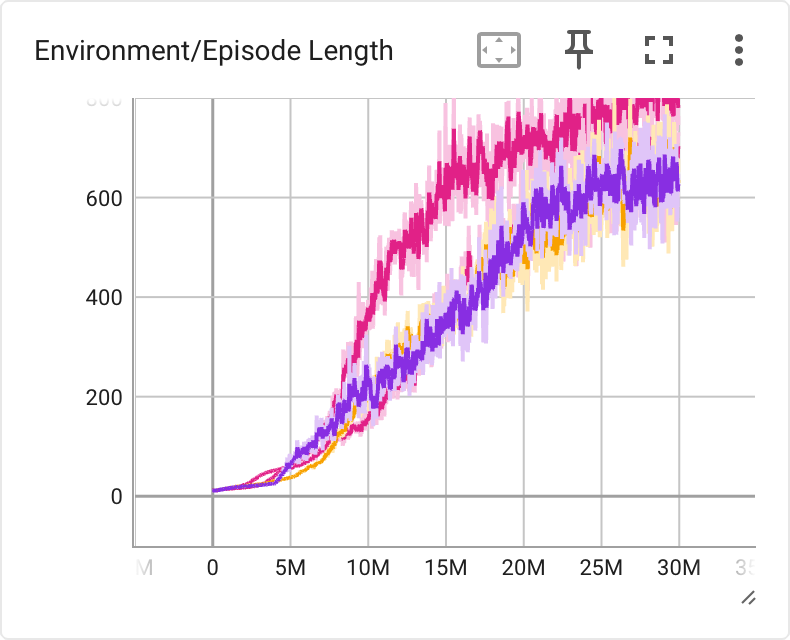
\includegraphics[width=\textwidth]{img/116_130_131_132_episode_length}
      \caption{Episodenlänge}
      \label{fig:116_130_131_132_episode_length}
    \end{subfigure}
    \begin{subfigure}{.49\textwidth}
      \centering  
      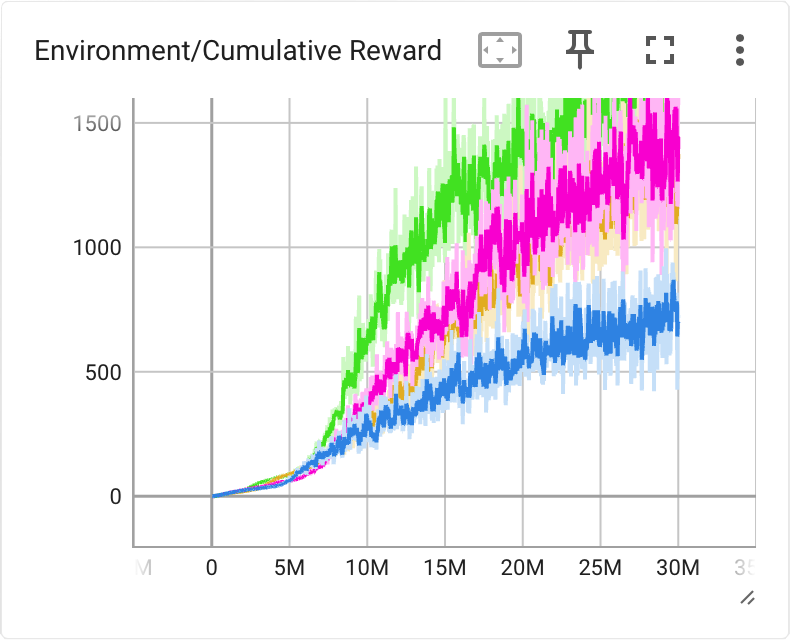
\includegraphics[width=\textwidth]{img/116_130_131_132_cumulative_reward}
      \caption{Angehäufte Belohnung}
      \label{fig:116_130_131_132_cumulative_reward}
    \end{subfigure}
     \begin{subfigure}{.49\textwidth}
      \centering  
      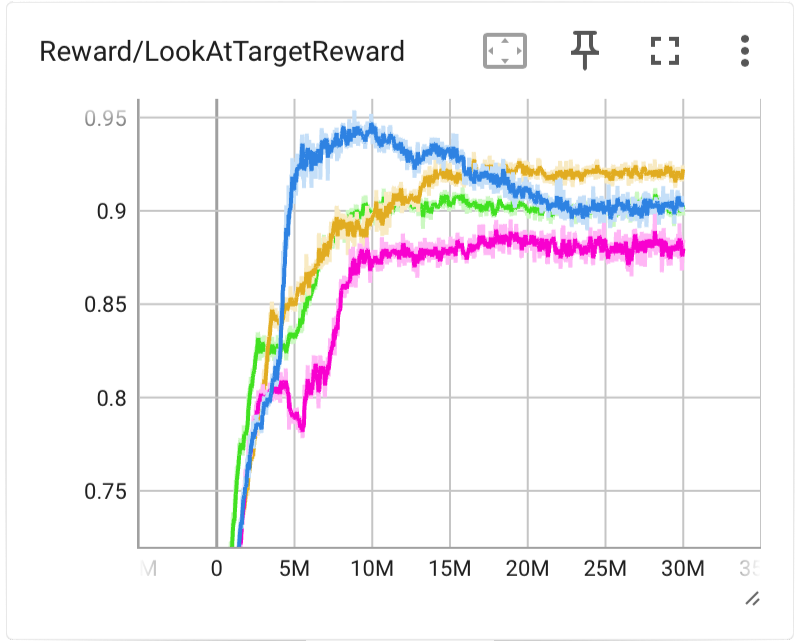
\includegraphics[width=\textwidth]{img/116_130_131_132_look_reward}
      \caption{Blickbelohnung}
      \label{fig:116_130_131_132_look_reward}
    \end{subfigure}
    \begin{subfigure}{.49\textwidth}
      \centering  
      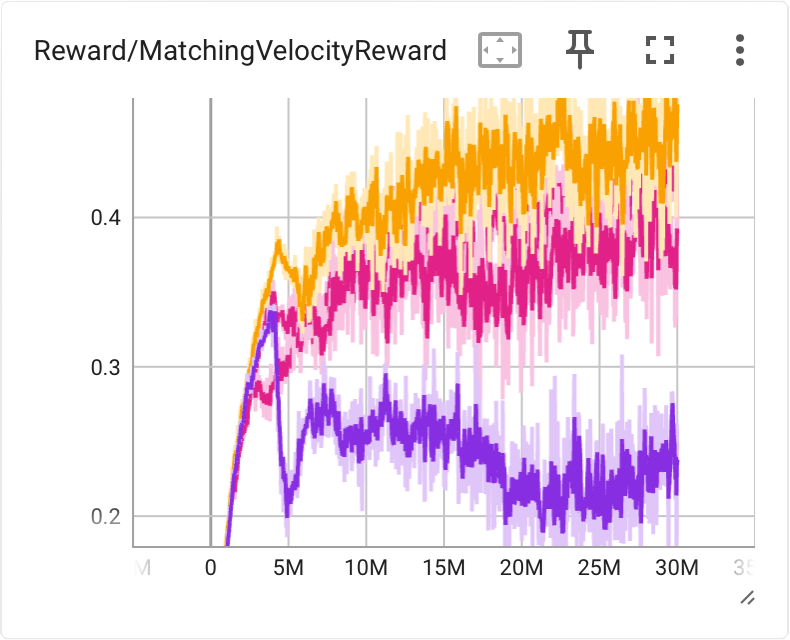
\includegraphics[width=\textwidth]{img/116_130_131_132_vel_reward}
      \caption{Geschwindigkeitsbelohnung}
      \label{fig:116_130_131_132_vel_reward}
    \end{subfigure}
    \begin{subfigure}{.49\textwidth}
      \centering  
      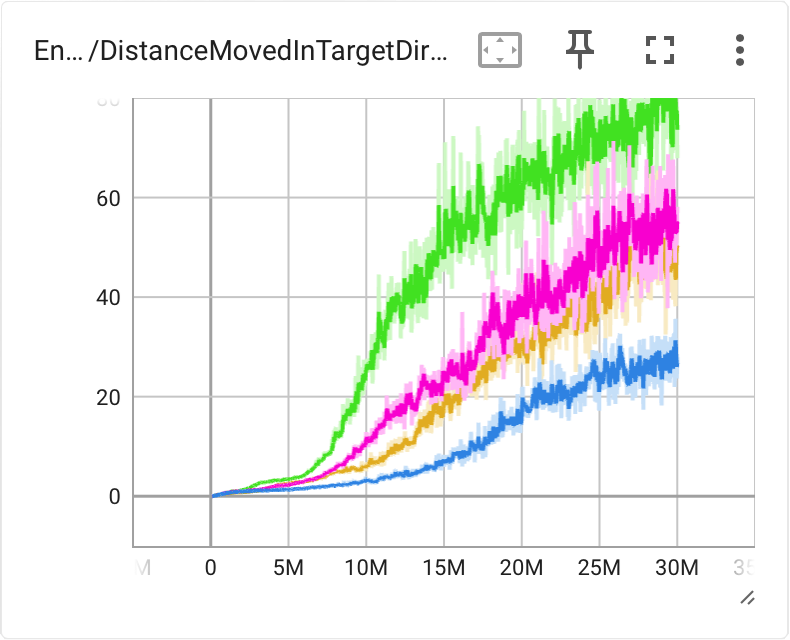
\includegraphics[width=\textwidth]{img/116_130_131_132_move_target_dir}
      \caption{Zurückgelegte Stecke in Zielrichtung}
      \label{fig:116_130_131_132_move_target_dir}
    \end{subfigure}
    \begin{subfigure}{.49\textwidth}
      \centering  
      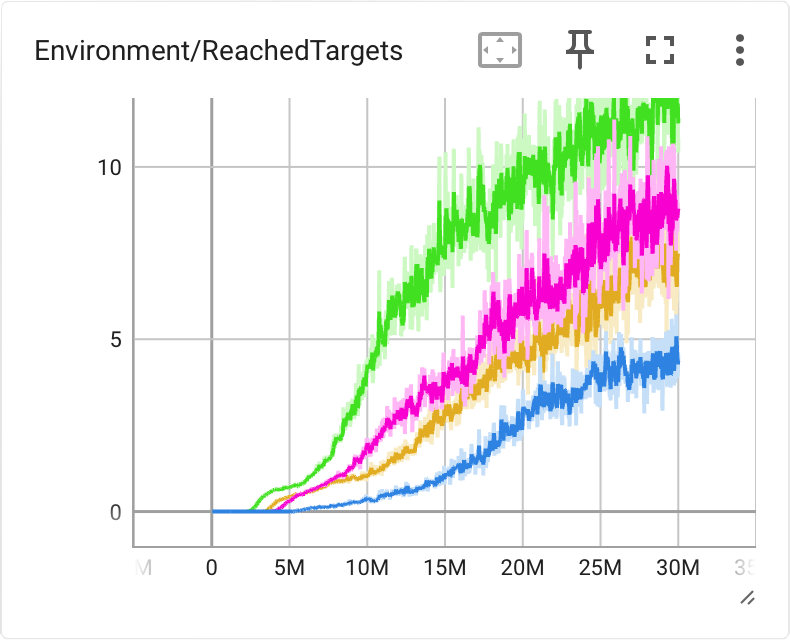
\includegraphics[width=\textwidth]{img/116_130_131_132_reach_target}
      \caption{Anzahl erreichte Ziele}
      \label{fig:116_130_131_132_reach_target}
    \end{subfigure}
  \caption{Unterschiedliche Blickrichtungen Training Graphen (grün = vorwärts, orange = rückwärts, rosa = rechts, blau = links)}
  \label{fig:training_unterschiedliche_blickrichtung}
\end{figure}